\begin{frame}[t]{C++: An evolving language}
\begin{center}
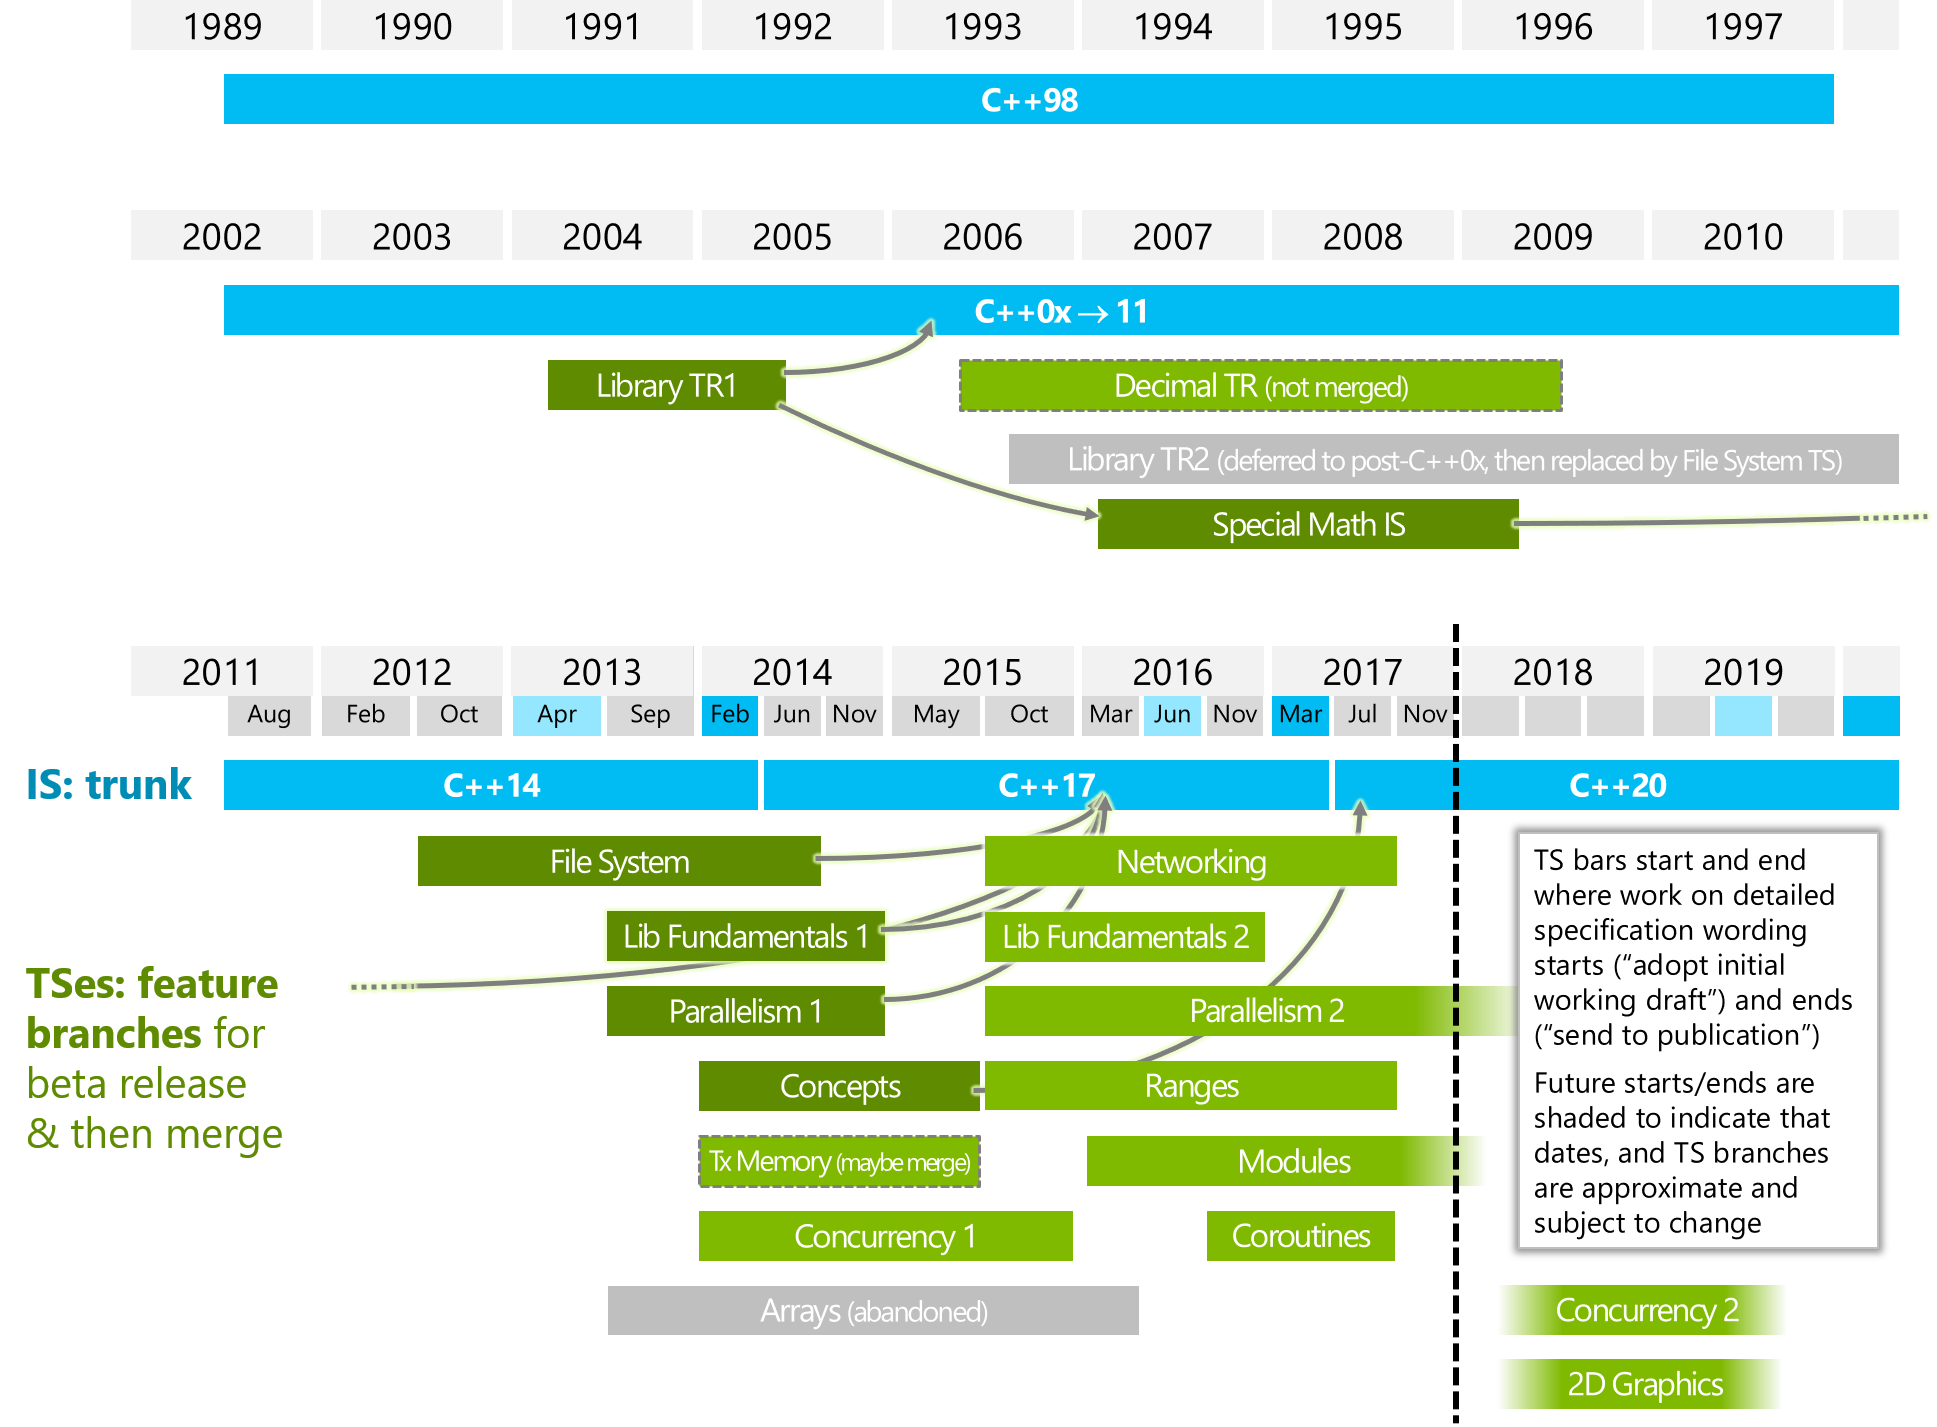
\includegraphics[height=.85\textheight]{img/wg21-timeline.png}
\end{center}
\end{frame}

\begin{frame}[t]{From C++98 to C++11}
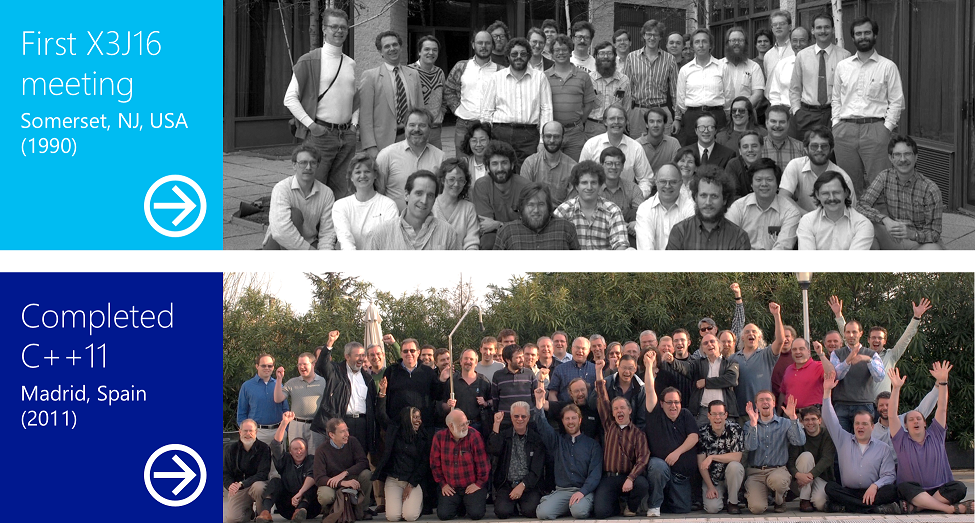
\includegraphics[width=\textwidth]{img/wg21-1990-2011.png}
\end{frame}

\begin{frame}[t]{C++14}
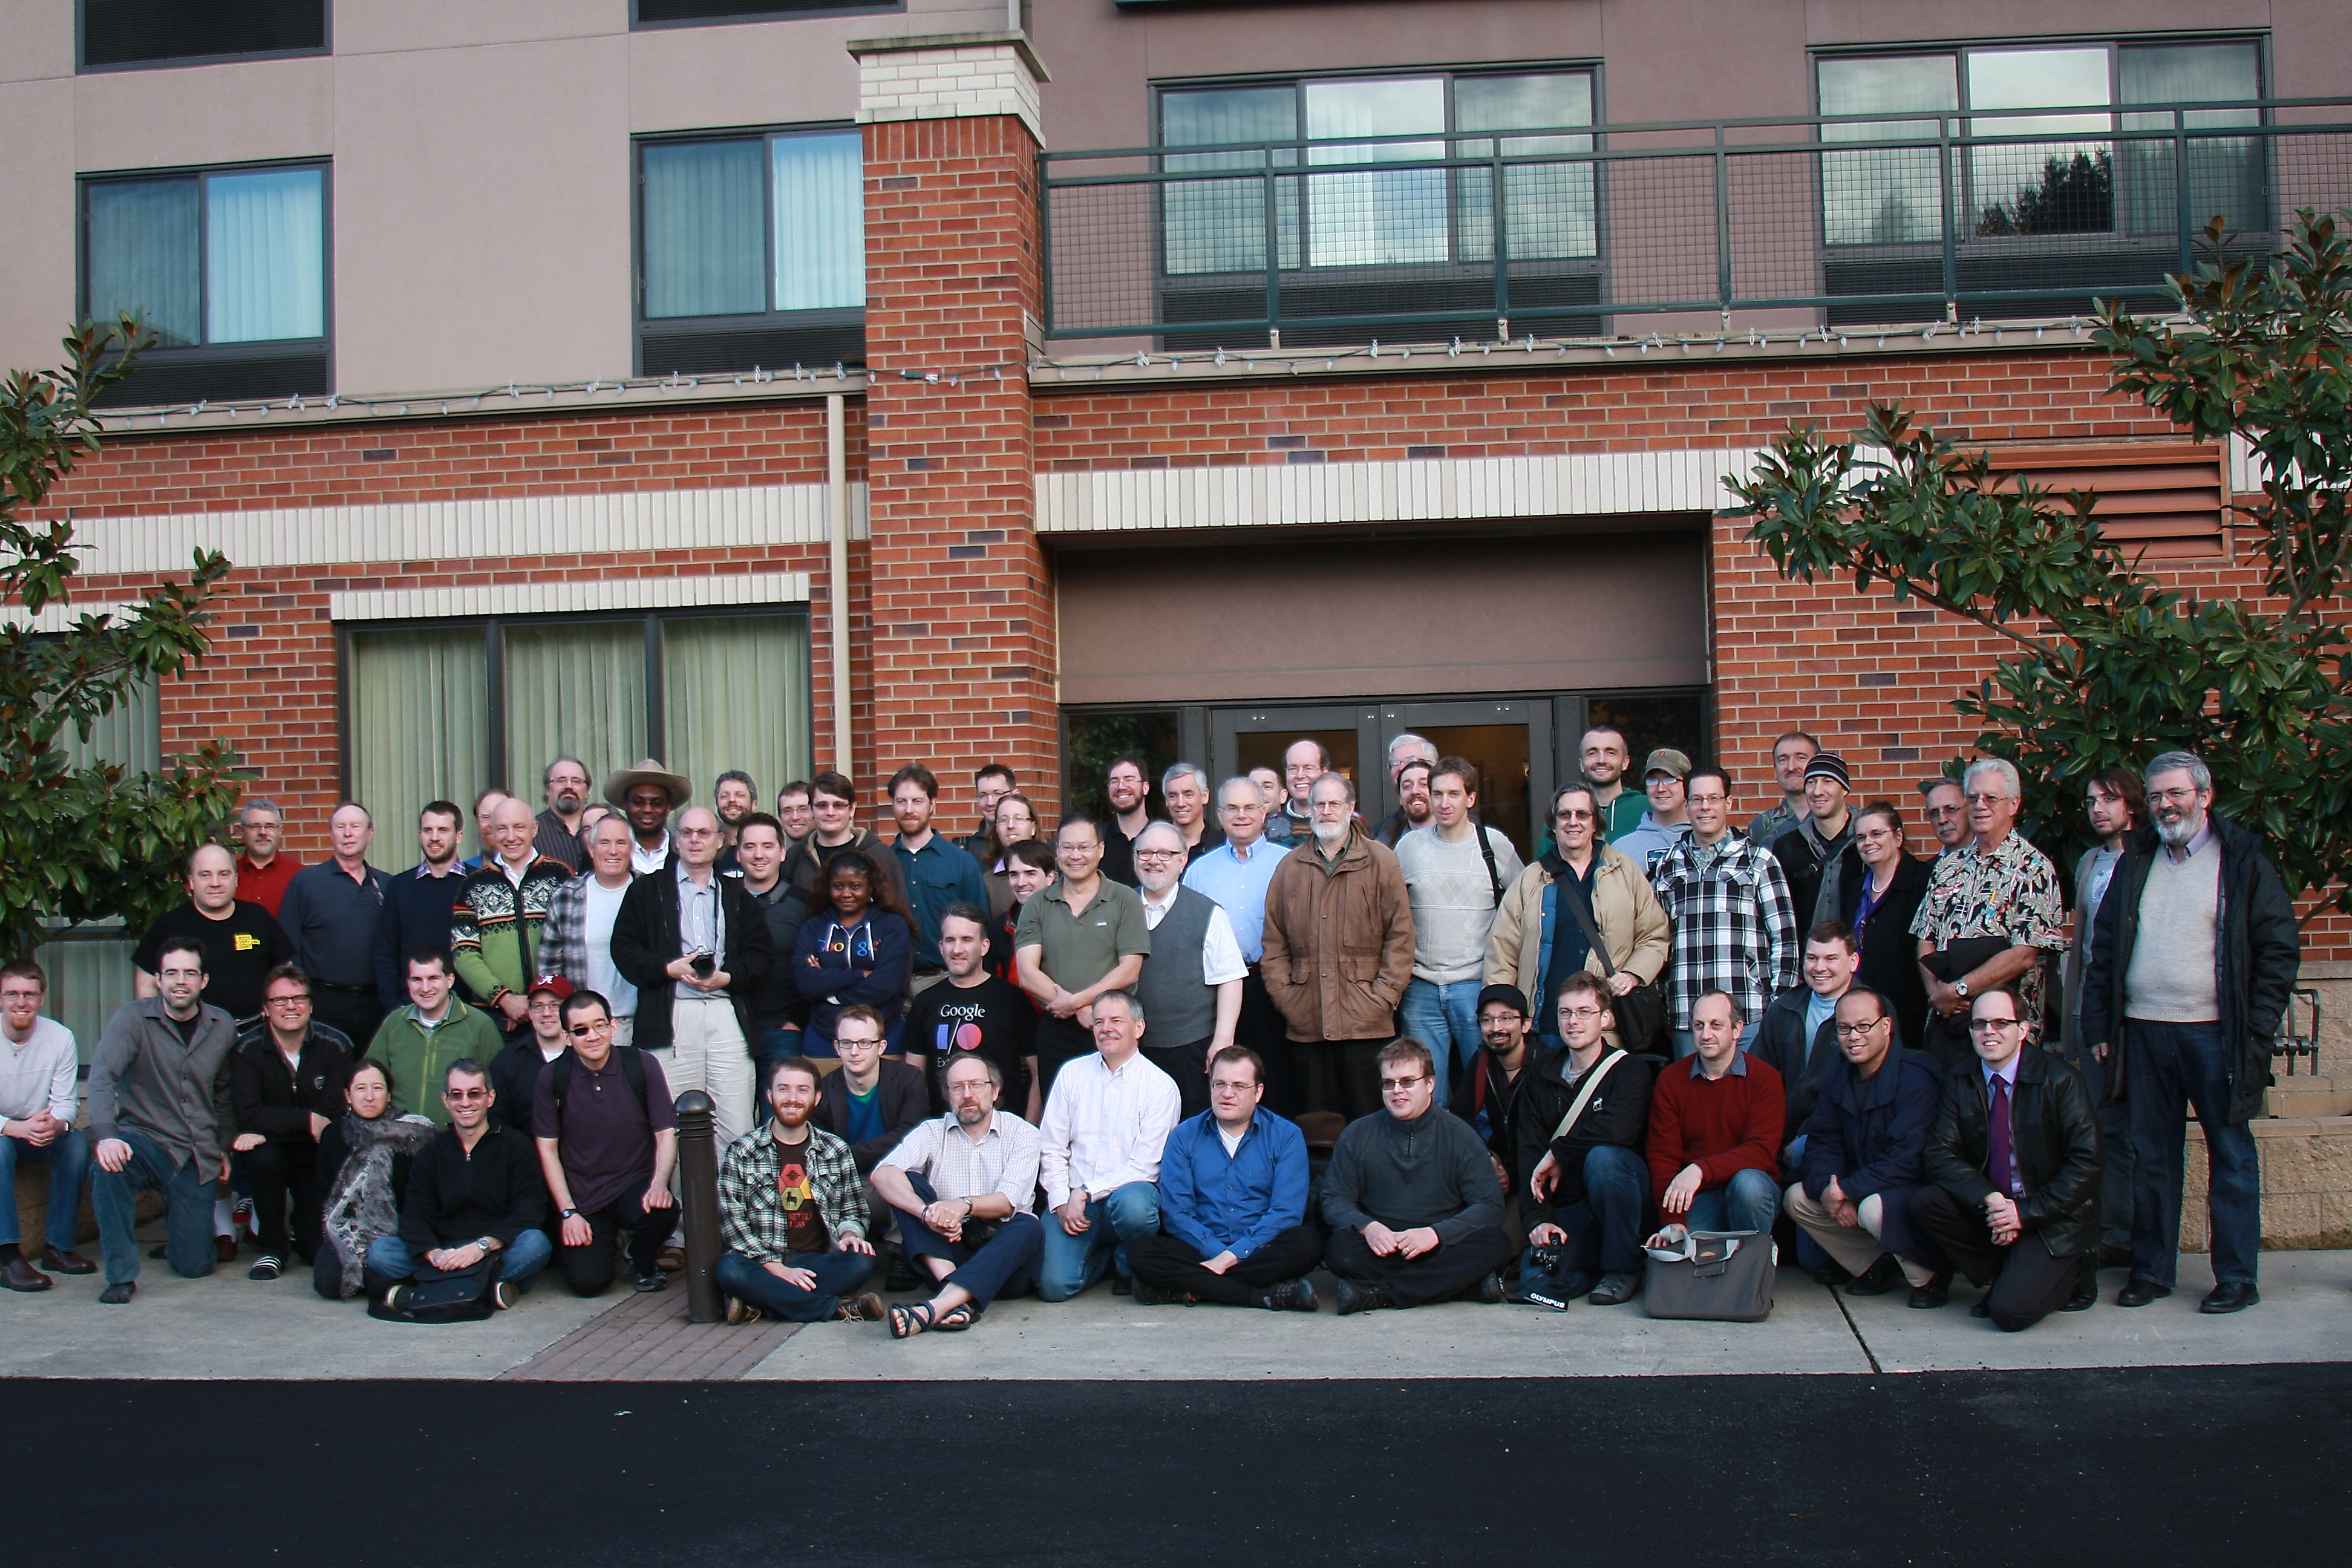
\includegraphics[width=\textwidth]{img/cpp-14.jpg}
\end{frame}

\begin{frame}[t]{C++17}
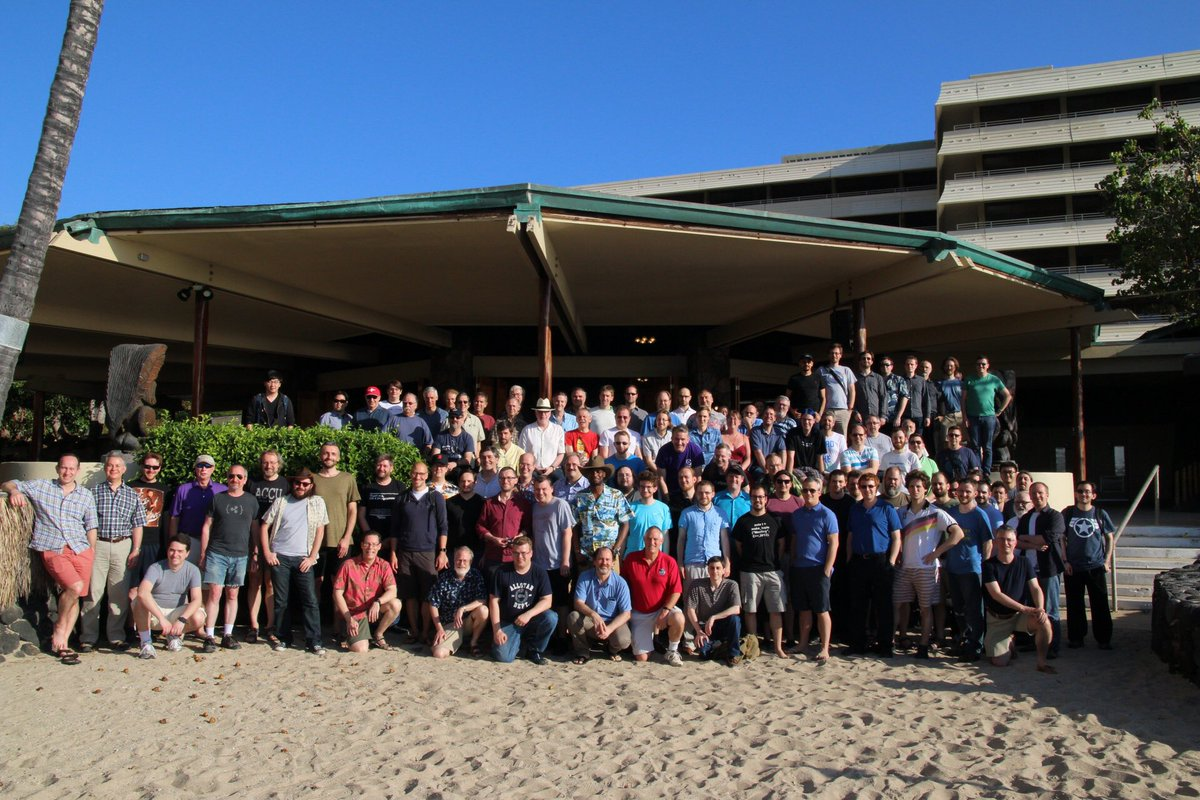
\includegraphics[width=\textwidth]{img/cpp-17.jpg}
\end{frame}

\begin{frame}[t]{What's new?}
\begin{itemize}
  \item Removing old stuff (e.g. trigraphs, \cppkey{register}, \cppid{auto\_ptr}, \ldots).
  \vfill\pause
  \item Clarifications (order of evaluation, copy elision, \ldots).
  \vfill\pause
  \item Better support for generic programming.
    \begin{itemize}
      \item Template argument deduction for classes.
      \item Expression folding.
      \item Compile time \cppkey{if}.
    \end{itemize}
  \vfill\pause
  \item Language simplifications:
    \begin{itemize}
      \item Structured binding.
      \item Initialization in \cppkey{if}/\cppkey{switch}.
    \end{itemize}
  \vfill\pause
  \item Library enhancements:
    \begin{itemize}
      \item \cppid{any}, \cppid{optional}, \cppid{variant}, \cppid{string\_view}.
      \item \cppid{filesystem}.
    \end{itemize}
  \vfill\pause
  \item \textbad{Parallel algorithms library}.
\end{itemize}
\end{frame}
